\documentclass[dvisvgm,tikz,border=4pt]{standalone}\usepackage{amsmath,amssymb}
\usetikzlibrary{arrows.meta,decorations.markings,backgrounds,cd,calc}
\colorlet{c1}{blue!70!black}\colorlet{c2}{red!70!black}\colorlet{c3}{green!45!black}
\tikzset{
 ->-/.style={decoration={markings,mark=at position .55 with {\arrow{Stealth[length=2.4mm]}}},postaction={decorate}},
 ->>-/.style={decoration={markings,mark=at position .5 with {\arrow{Stealth[length=2.4mm]}},mark=at position .6 with {\arrow{Stealth[length=2.4mm]}}},postaction={decorate}},
 every picture/.append style={show background rectangle, background rectangle/.style={fill=white}}
}

\begin{document}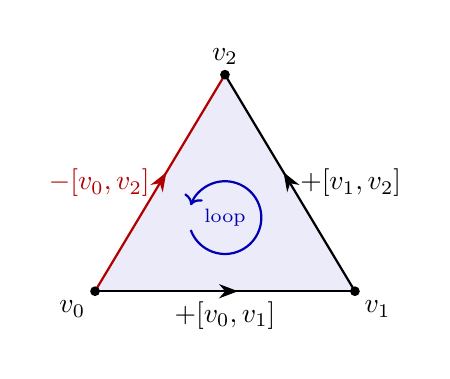
\begin{tikzpicture}[scale=1.1]
\coordinate (A) at (0,0); \coordinate (B) at (3,0); \coordinate (C) at (1.5,2.5);
\fill[c1!8] (A)--(B)--(C)--cycle;
\draw[thick,->-] (A)--(B) node[midway,below]{$+[v_0,v_1]$};
\draw[thick,->-] (B)--(C) node[midway,right]{$+[v_1,v_2]$};
\draw[thick,->-,c2] (A)--(C) node[midway,left]{$-[v_0,v_2]$};
\foreach \p/\n/\pos in {A/v_0/below left,B/v_1/below right,C/v_2/above}{\fill (\p) circle(1.6pt) node[\pos]{$\n$};}
\draw[->,c1,thick] (1.5,0.85) ++(200:0.42) arc[start angle=200,end angle=520,radius=0.42];
\node[c1,font=\scriptsize] at (1.5,0.85) {loop};
\end{tikzpicture}\end{document}
